\documentclass[9pt,a4paper]{article}

%-------------------------------%
% Commands and packages
\usepackage{amsmath,amssymb,bm,physics,graphicx,hyperref}
\usepackage[left=5mm, right=5mm, top=5mm, bottom=10mm]{geometry}
\usepackage{subcaption}

%CUSTOM COMMANDS
\renewcommand{\Re}{\mathbf{re}}
\renewcommand{\Im}{\mathbf{im}}
\newcommand{\R}{\mathbb{R}}
\newcommand{\N}{\mathbb{N}}
\newcommand{\C}{\mathbb{C}}
\newcommand{\lap}{\mathscr{L}}
\DeclareMathOperator{\atantwo}{atan2}


\hypersetup{
    colorlinks = true,  %Colours links instead of ugly boxes
    urlcolor   = blue,  %Colour for external hyperlinks
    linkcolor  = black, %Colour of internal links
    citecolor  = black  %Colour of citations
}

%-------------------------------%
% Main document
\begin{document}
    \thispagestyle{empty}
    \numberwithin{equation}{section}
    \numberwithin{table}{section}
    \section{Dynamic System Analysis} \label{Sec1}
    The aircraft system dynamics is described by the following system of differential equations (which are linear and in state space representation). State variables are $\alpha, r, \theta$ and input is $\delta$.
    \begin{equation*}
        \dot{\alpha} = -0.31\alpha + 57.4r +0.232\delta, \quad
        \dot{r} = -0.016\alpha-0.425r+0.0203\delta, \quad
        \dot{\theta} = 56.7r.
    \end{equation*}
    For open-loop dynamics, we must take into account the impact of the actuator and sensor. From the question sheet, their respective transfer functions are

    $$G_{a}(s)=\frac{1}{0.0145s+1}, \; \; G_{m}(s)=\frac{e^{-0.0063s}}{0.0021s+1}.$$
    
    \noindent The actuator has a pole at $s = -\frac{1}{0.0145}$, while the sensor has one at $s=-\frac{1}{0.0021}$; both have negative real parts. Since the open-loop system is the cascade of actuator, aircraft dynamics, and sensor transfer functions, as shown in the block diagram in Figure \ref{fig:ol_blockDiagram}, if the transfer function for aircraft dynamics ($G_{\alpha}, G_{r}, \text{or } G_{\theta}$) has only poles with negative real parts, the open-loop system is stable \cite[Theorem 9.9]{textbook}.
    \begin{figure}[h]
        \begin{subfigure}[h]{0.5\textwidth}
            \centering
            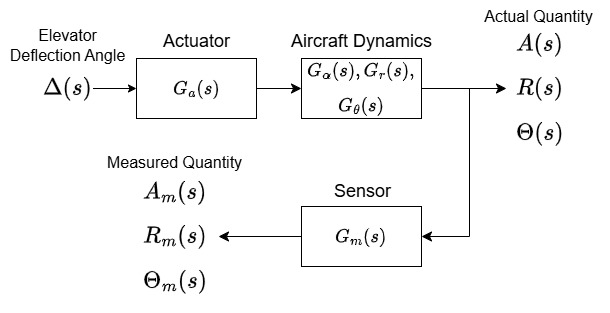
\includegraphics[width = \textwidth]{figs/ELE2038_H5_openLoopBlockDiagram.drawio.jpg}
            \caption{Open-loop system for all 3 states.}
            \label{fig:ol_blockDiagram}            
        \end{subfigure}%
        \begin{subfigure}[h]{0.5\textwidth}
            \centering
            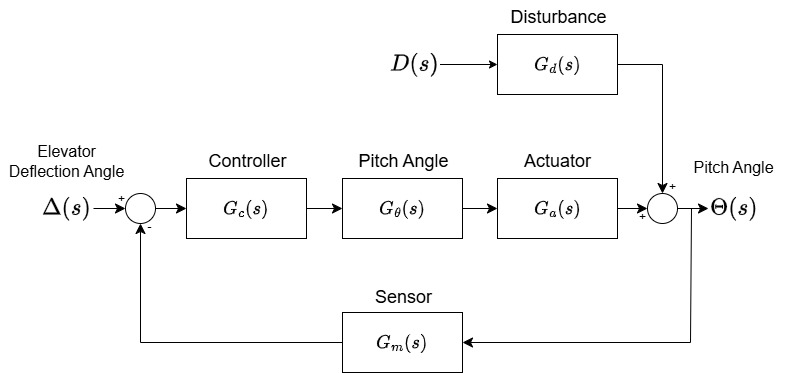
\includegraphics[width = \textwidth]{figs/ELE2038_H5_closedLoopBlockDiagram.drawio.jpg}
            \caption{Closed-loop system for pitch angle.}
            \label{fig:cl_blockDiagram}
        \end{subfigure}
    \caption{Block diagrams relating deflection angle of elevators to angle of attack, pitch rate, and pitch angle.}
    \end{figure}
    
    \noindent Assuming zero initial conditions, the Laplace transform can be applied to the differential equations given in Section \ref{Sec1} to find
    \begin{subequations}
        \begin{align}
            G_\alpha =\frac{A(s)}{\Delta(s)}= & \frac{0.232s + 1.26382}{(s + 0.31)(s + 0.425) + 0.9184}, \\
            G_r =\frac{R(s)}{\Delta(s)}=& \frac{0.0203s + 0.002581}{(s + 0.31)(s + 0.425) + 0.9184}, \\
            G_\theta =\frac{\Theta(s)}{\Delta(s)}=& \frac{1.15101s + 0.1463427}{s((s + 0.31)(s + 0.425) + 0.9184)}.
        \end{align}
    \end{subequations}
    The poles of $G_\alpha$ and $G_r$ are $s=-0.3675 \pm j0.9566$, which have negative real parts, therefore the open-loop system corresponding to each of these two states is BIBO stable (the open-loop impulse, step, and frequency response of these systems can be found in the linked Python notebook \cite{python_notebook}). Since $G_{\theta}(s)=\frac{56.7}{s}G_{r}(s)$; $G_{\theta}$ shares all poles of $G_{r}$, which are all stable, but also possesses an additional pole at $s=0$. Since we have a pole with a non-negative real part, $G_{\theta}$ is not BIBO stable, meaning the open-loop system relating the deflection angle of elevators to the pitch angle is also not BIBO stable; a controller is required.

    
    \begin{figure}
    \centering
        \begin{subfigure}[h]{0.35\textwidth}
            \centering
            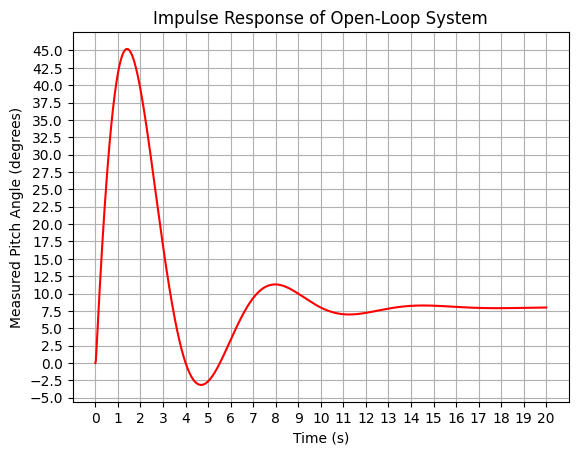
\includegraphics[width = \textwidth]{figs/GthetaImpRes.png}
            \caption{Impulse response.}
            \label{fig:gThetaImpRes}
        \end{subfigure}%
        \begin{subfigure}[h]{0.35\textwidth}
            \centering
            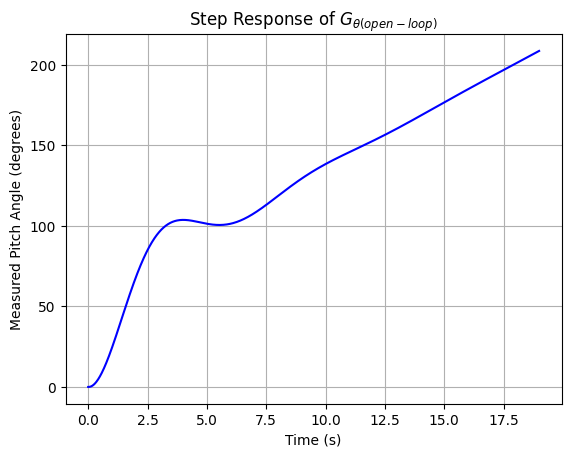
\includegraphics[width = \textwidth]{figs/GthetaStepRes.png}
            \caption{Step response.}
            \label{fig:gThetaStepRes}
        \end{subfigure}
    \caption{Open-loop system responses for pitch angle of the aircraft, with transfer function $G_{\theta(\text{open-loop})}=G_{\theta}G_{a}G_{m}$.}
    \end{figure}

    
    Figures \ref{fig:gThetaImpRes} and \ref{fig:gThetaStepRes} show the impulse and step response of this unstable system. As expected, the pitch angle does not return to zero for the impulse response and does not converge to any value, but rather increases indefinitely for the step response. Frequency response of $G_{\theta(\text{open-loop})}$ may also be found in the Python notebook \cite{python_notebook}.

    \section{Implementing and Tuning a Controller for the Pitch Angle}
    We will use a PID controller to give zero offset and to dampen oscillations in system responses as an aircraft requires precise and smooth behaviour. The block diagram of the closed-loop system is shown in Figure \ref{fig:cl_blockDiagram}, where $G_{c}=K_{c}(1+\tau_{D}s+\frac{1}{\tau_{I}s})$. The closed-loop transfer function is then $$G_{\text{cl}}=\frac{G_cG_aG_\theta}{1+G_cG_aG_\theta G_m}.$$ To allow analysis of the system in the control library, we use a Padé approximation of the exponential in the sensor transfer function \cite[Section 9.4]{textbook}. Using Ziegler-Nichols ultimate sensitivity method (ZNUS) \cite[Section 10.3.3]{textbook} for tuning, we find $K_u=23.38$ and $T_u=1.1982$, and therefore $K_c=14.028$, $\tau_D=0.150$, and $\tau_I=0.599$. In the Python notebook \cite{python_notebook}, the impulse, step, and frequency response of this system is simulated and shows $\text{rise time}=0.236$ seconds, $\text{settling time}=7.308$ seconds, and $\text{overshoot}=62.17\%$. With the aim of improving these metrics, while also avoiding overly aggressive responses, we will further tune the controller manually. Through experimentation, $K_c=14.028$, $\tau_D=0.16$, and $\tau_I=2$ have been deemed adequate for this controller.

    \begin{figure}[!ht]
        \centering
        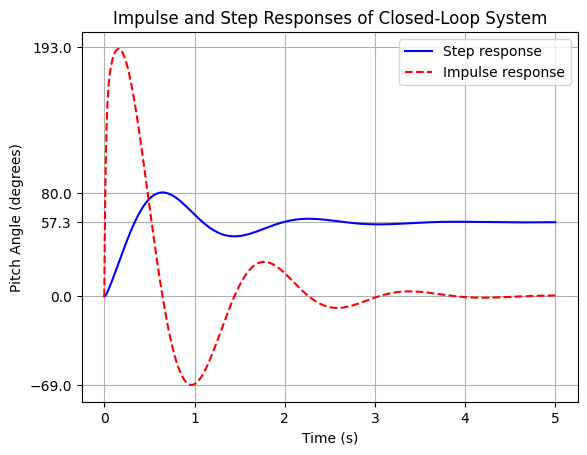
\includegraphics[width=0.35\linewidth]{figs/Fig3CLTFImpStep.png}
        \caption{Impulse and step response of the closed-loop system for pitch angle with a manually tuned PID controller.}
        \label{fig:3}
    \end{figure}

    \noindent By increasing $\tau_I$ and $\tau_D$ we reduce the overshoot, which now becomes $40.59\%$. Settling time is also reduced from $7.3$ seconds to $3.2$ seconds, making this manually tuned controller more appropriate for aircraft pitch control than the one tuned using ZNUS. The offset of the system has been proven to be zero in the Python notebook \cite{python_notebook}, and this can also be seen visually in Figure \ref{fig:3}.

    \section{System Response to Disturbances}
    Possible disturbances for an aircraft system include wind gusts (modelled as a unit step) and turbulence (modelled as a unit impulse). We will test the system with a disturbance transfer function $G_d = \frac{K}{\tau s + 1}$ where $K = \tau = 1$, with reference to Figure \ref{fig:cl_blockDiagram}. The load transfer function is given by
    \begin{equation}
        G_{L}(s) = \frac{\Theta(s)}{D(s)} = \frac{G_d}{1 + G_c G_a G_\theta G_m}.
    \end{equation}
    Evaluating poles of $G_L$ in Python we find that all poles have negative real parts except for two poles at the origin, meaning the load transfer function is not BIBO stable and the closed-loop system has poor disturbance rejection. The impulse and step response for disturbances in the closed-loop system can be found in the Python notebook \cite{python_notebook}.

    \section{Bode Stability Criterion and Stability Margins}
    For a closed-loop transfer function to be BIBO stable, the corresponding open-loop transfer function must meet the conditions outlined in Bode Stability Criterion \cite[Theorem 11.6]{textbook}. To verify the first criteria, we find the poles of the open-loop system; in the Python notebook \cite{python_notebook} it has been shown that the poles all have a negative real part except for one that is at the origin, satisfying the first criteria. To confirm the other criteria, Bode plots of the open-loop system are included in the Python notebook \cite{python_notebook}, from which we can conclude that there are crossover frequencies at $\omega_{\text{co,0}}=63, \; \omega_{\text{co,1}} = 630$, and $\omega_{\text{co,2}} = 1412$; satisfying criteria 2. By further inspection of the Bode plots we see that $|G_{\text{ol}}(j\omega_{co,k})| < 1$ for $k=0, 1, 2$ satisfying criteria 3. All 3 criterion are satisfied, therefore the proposed closed-loop system is BIBO stable. 
    
    
    In the Python notebook \cite{python_notebook}, we have used Bode plots while applying various different values of additional gain and time delay to the system to find $\text{gain margin GM} = 29.5$ dB, $\text{delay margin DM} = 0.15$ seconds, and $\text{phase margin PM} = \omega_g\text{DM}=21.6^\circ$, where $\omega_g=2.51$ is the frequency in the Bode plot which satisfies $|G_{\text{ol}}(j\omega_g)|=1$. The system is stable even when a large additional gain is introduced, and has adequate stability when faced with small time delays, although a larger delay margin would be advantageous to make the system less likely to become unstable when additional time delay arises.

    \thispagestyle{empty}

    % BIBLIOGRAPHY %%%%%%%%%%%%%%%%%%%%%%%%%%%%%%%%%%%%%%%%%%%%%%%%%%%
    \bibliographystyle{IEEEtran}
    \bibliography{references.bib}
    
\end{document}